\documentclass[12pt,a4paper]{article}
\usepackage[italian]{babel}
\usepackage[T1]{fontenc}
\usepackage[latin1]{inputenc}
\usepackage{graphicx}
\usepackage{amsmath}
\usepackage{subfig}
\date{}
\begin{document}
\title{Strutture Aeronautiche\\ Esercitazione 4 \\ Prof.re Franco Mastroddi}
\author{Matteo Hakimi 1455230}
\maketitle
\begin{figure}[htbp]
\centering

\includegraphics[width=100mm]{Immagini/1}
\end{figure}
\newpage
\tableofcontents
\newpage


\section{Introduzione}
Si vogliono calcolare gli stress indotti, attraverso un codice agli elementi finiti, delle seguenti strutture:\\ \\
\textbullet \quad Cilindro infinito pressurizzato\\ \\
\textbullet \quad Calotta sferica pressurizzata soggetta al proprio peso\\ \\
\textbullet  \quad Calotta sferica con apertura polare soggetta a carico anulare sulla sommit\'a e peso proprio\\ \\
Si effettuer\'a inoltre il confronto con la soluzione ottenuta per via analitica.\\
Infine saranno calcolati, sempre con l'utilizzo di un solutore Fem, i modi propri di vibrazione della calotta con e senza apertura polare.
\section{Cilindro infinito pressurizzato}
Il primo caso analizzato \'e quello del cilindro infinito cavo in lega leggera (alluminio), di raggio $r=2.5 m$ e spessore $t=2.5 mm$ chiuso alle estremit\'a,�pressurizzato con pressione $p=150kPa$ .\\
\begin{figure}[htbp]
	\centering
	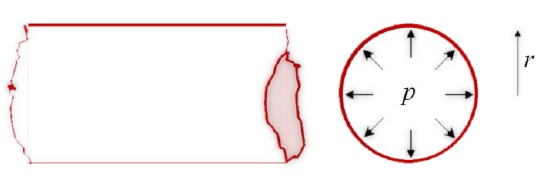
\includegraphics[scale=0.4]{Immagini/Cilindro.jpg}
	\caption{Cilindro pressurizzato}
\end{figure}
Dalla teoria analitica dei gusci sottili, avendo definito un sistema di coordinate cilindriche (r $\theta$ x), gli stress normali $\sigma_{\theta}$ e $\sigma_{x}$   sono dati da:\\ \\
\textbullet \quad $\sigma_{\theta}=\dfrac{pr_{0}}{t}= 150 Mpa $\\ \\
\textbullet \quad $\sigma_{x}=\dfrac{pr_{0}}{2t}= 75 Mpa $\\ \\
Data l'impossibilit\'a di implementare su software una struttura "infinita", in prima approssimazione il problema pu\'o essere diviso in due sottoproblemi di natura pi\'u semplice, poich\'e,  il caso analizzato presenta particolari simmetrie a meno di effetti di bordo.\\
Si proceder\'a quindi con l'implementazione e lo studio dei due sottocasi:\\ \\
\textbullet \quad Cilindro finito aperto con pressione interna libero-libero\\ \\
\textbullet \quad Cilindro finito aperto soggetto a carico di trazione sul bordo incastrato-libero\\ \\
Bisogna notare che un modo alternativo di procedere,al fine di ottenere una soluzione pi\'u simile possibile a quella analitica, \'e quello di considerare un cilindro finito chiuso pressurizzato e controllare lo stress in prossimit\'a della sezione centrale.
\subsection{Cilindro finito pressurizzato}
Il cilindro viene modellato finito aperto alle estremit\'a, soggetto a una pressione interna, avendolo oppurtanamente discretizzato con 40 elementi in direzione circonferenziale e 30 in direzione longitudinale, per un totale di 1200 elementi SHELL.\\
Imponendo come condizioni al contorno uno spostamento di estremit\'a in direzione longitudinale uguale e contrario a quello della faccia opposta, si ha che la $\sigma_{\theta}$ ottenuta con solutore FEM \'e pari a:\\
\textbullet\quad$\sigma_{\theta}=1.495376E+08 Pa$\\
costante in tutte le sezioni e nello spessore.\\
Si ottiene cio\'e una soluzione molto prossima a quella ottenuta per via analitica ipotizzando uno sforzo solamente di natura membranale.\\
Data l'assenza di $\sigma_{x}$ si prevede una deformazione $\epsilon_{\theta}=\dfrac{\sigma_{\theta}}{E}=2.143$ $10^{-3}$ ovvero uno spostamento in direzione radiale $\Delta r= 5.357$ $10^{-3} m$, in buon accordo con quello attenuto con solutore $\Delta r_{FEM}= 5.340630E-03 m$\\
Per completezza si riporta la deformata ottenuta tramite codice FEM.
   \begin{figure}[htbp]
   	\centering
   	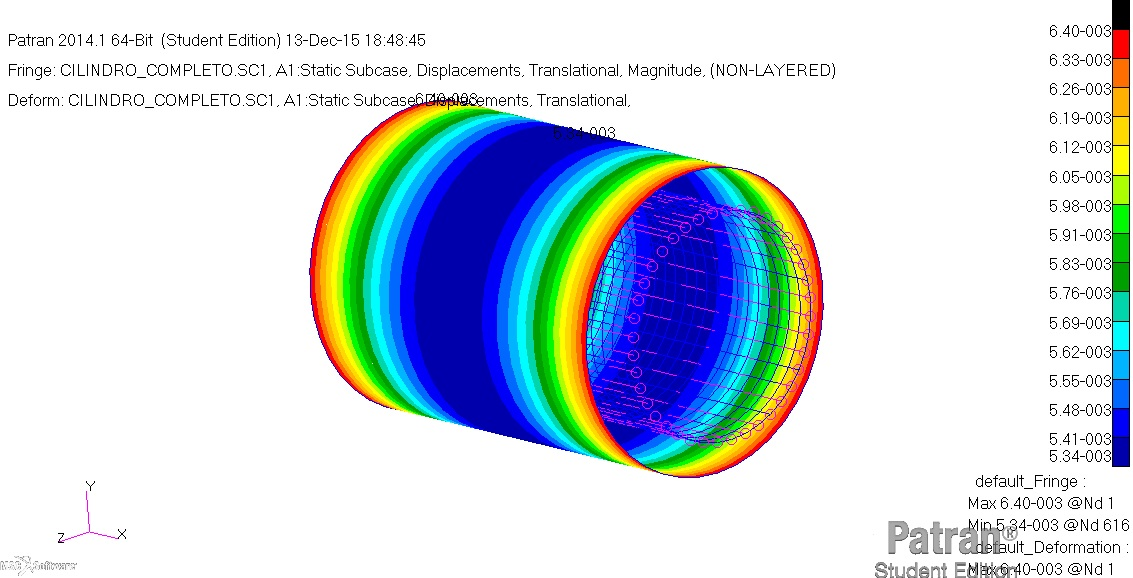
\includegraphics[scale=0.4]{Immagini/Cilindroin.jpg}
   	\caption{Deformata cilindro}
   \end{figure}
\newpage
\subsection{Cilindro finito caricato sul bordo}
Al fine di considerare gli effetti membranali dovuti alla pressione agente sulle basi del cilindro, mantenendo la stessa discretizzazione del caso precedente (40 x 30 elementi SHELL), viene incastrata una  delle estremit\'a e viene applicato un carico di trazione uniformemente ditribuito sull'altra; caricando direttamente ogni nodo della faccia con una forza di intensit\'a pari a $F=\dfrac{p \pi r^2 }{2 \pi r N_{Nodi}}$ dove $N_{Nodi}$ \'e il numero di nodi sulla faccia stessa .\\
Si noti che in questo caso non si sta modellizzando il coperchio che chiude la faccia d'estremit\'a, ma piuttosto l'effetto del coperchio stesso, che induce uno stato di stress $\sigma_{x}$ in direzione assiale.\\
Procedendo con il calcolo si ottiene:\\
\textbullet \quad $\sigma_{x}=7.507616E+07 Pa$\\
Anche in questo caso si nota un buon accordo con la soluzione ottenuta analiticamente; inoltre si ha $\Delta r=-\nu \sigma_{x} r_{0}$ $-0.803$ $10^{-3} m$ mentre quella  ottenuta tramite software \'e $\Delta r_{FEM}= -0.786635E-03$; si noti come la somma dei spostamenti complessivi in direzione radiale, ottenuti analiticamente, siano in buon accordo con quelli ottenuti tramite codice FEM: $\Delta r_{tot}= 4.554$ $10^{-3} m$  $\Delta r_{FEM tot}= 4.554$ $10^{-3} m$.\\
Infine, anche in questo caso, si riporta la deformata ottenuta tramite solutore.
  \begin{figure}[htbp]
  	\centering
  	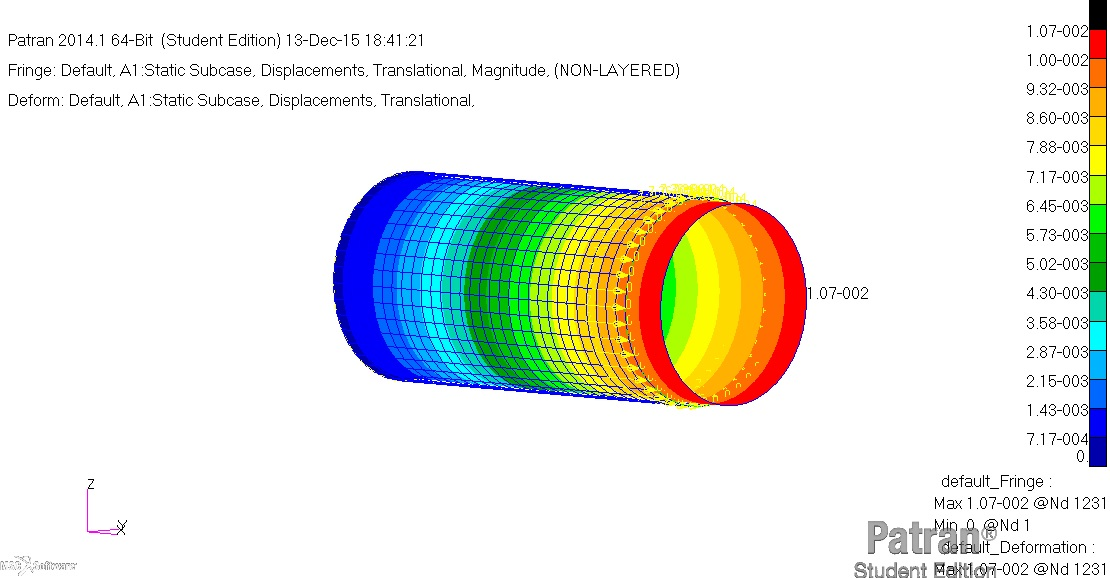
\includegraphics[scale=0.4]{Immagini/Cilindrof.jpg}
  	\caption{Deformata cilindro}
  \end{figure}
     \newpage

\section{Calotta sferica pressurizzata soggetta al peso proprio}
Il caso successivo riguarda la determinazione della risposta statica di una cupola sferica, appoggiata sul bordo, troncata  ($\alpha= 60�$ si veda figura) in alluminio, di spessore $t=2.0$ $10^{-3} m$ e raggio $r= 1 m$ pressurizzata $p=75kPa$  e soggetta al proprio peso.\\
 \begin{figure}[htbp]
 	\centering
 	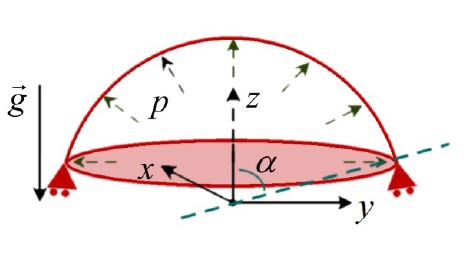
\includegraphics[scale=0.4]{Immagini/Cupola.jpg}
 	\caption{Calotta}
 \end{figure}\\
 Per la cupola pesante pressurizzata la soluzione analitica fornisce i seguenti risultati:\\ \\
\textbullet \quad Pressione interna: $\sigma_{\theta}=\sigma_{\phi}=\dfrac{p\cdot r}{2\cdot t}$\\ \\
\textbullet  \quad Gravit\'a: $\sigma_{\phi}=\dfrac{\overline{p}r}{t(1+\cos\phi)}$, $\sigma_{\theta}=\dfrac{\overline{p}r}{t} ( \dfrac{1}{1+\cos\phi}-\cos\phi )$\\ \\ dove $\overline{p}$ \'e la forza peso per unit\'a di superficie della calotta, $\overline{p}=\rho\cdot g\cdot t $.\\ 
Al fine di calcolare la soluzione mediante solutore FEM si \'e proceduto con la discretizzazione della struttura come segue:\\ \\
\textbullet \quad Suddivisione di ogni parallelo con 30 elementi SHELL \\ \\
\textbullet \quad Suddivisione di ogni meridiano con 120 elementi SHELL\\ \\
In particolare gli elementi scelti al fine di eseguire la mesh sono di tipo eterogeneo (CQUAD4, CTRIA3). \\
 Si noti come gli elementi di tipo CTRIA3 sono stati collocati in prossimit\'a del polo, e come questi risultino essere di dimensione minore rispetto a quelli di tipo CQUAD4, questo perch\'e, data la particolare geometria di questi elementi si riesce a ricoprire perfettamente la superficie in prossimit\'a del polo. Tuttavia gli elementi di tipo CTRIA3 forniscono un campo di deformazione (e quindi di stress) costante all'interno dell'elemento, per questo motivo si \'e proceduto con l'infittimento locale nell'intorno del polo.\\
 Inoltre \'e stato creato un elemento RBE3 che vincola il nodo all'apice della cupola a muoversi solidarmente ai nodi del parallelo adiacente, questo perch\'e sempre in prossimit\'a del polo si verifica un affossamento della cupola che nella realt\'a non si verifica.\\
 Si procede ora con il calcolo della soluzione, analizzando separatamente i diversi contributi del carico (solamente gravit\'a e solamente pressione) e poi globalmente.  
 \subsection{Calotta sferica pressurizzata}
 Il primo sottocaso analizzato \'e quello inerente alla struttura solamente pressurizzata.\\
 Ricordiamo che la teoria analitica dei gusci sottili, avendo considerato un campo di sforzo puramente membranale \'e dato da:\\ \\
\textbullet \quad $\sigma_{\theta}=\sigma_{\phi}=\dfrac{p\cdot r}{2\cdot t}=18.75 MPa$ \\ \\
 Si riportano i risultati ottenuti per l'elemento 413 della struttura\\
 \begin{center}
 	\begin{tabular}{c c}
 		\hline	
 $\sigma_{\theta_{+}}$ & $1.874015E+07 Pa$\\
 \hline
 $\sigma_{\theta{-}}$ & $ 1.874026E+07 Pa$\\
 \hline
 $\sigma_{\phi_{+}}$ & $  1.873922E+07  Pa$\\
 \hline
 $\sigma_{\phi_{-}}$ & $  1.873958E+07   Pa$\\
        	\hline
 \end{tabular}
\end{center} 
 Avendo indicato con + lo sforzo sulle fibre superiori dello spessore e con - quello inferiore.
 Si osserva una variazione di stress nello spessore pari a $\Delta \sigma_{\theta}=0.000011 Pa$ e $\Delta \sigma_{\phi}=0.00036 Pa$.\\
 Si nota come i risultati ottenuti attraverso solutore FEM siano in ottimo accordo con quelli ottenuti analiticamente, avendo considerato solamente uno sforzo puramente membranale.
 \subsection{Calotta sferica soggetta al peso proprio}
 Si passa ora al calcolo del campo di stress della struttura soggetto al peso proprio. \\
 Dalla teoria analitica dei gusci sottili si ha che:\\ \\
 \textbullet \quad $\sigma_{\phi}=\dfrac{\overline{p}r}{t(1+\cos\phi))}$\\ \\
 \textbullet \quad $\sigma_{\theta}=\dfrac{\overline{p}r}{t}( \dfrac{1}{1+\cos\phi}-\cos\phi)$\\ \\
 Si osserva come in questo caso la tensione meridiana e quella parallela varino in funzione della colatitudine $\phi$.
 \begin{figure}[htbp]
 	\centering
 	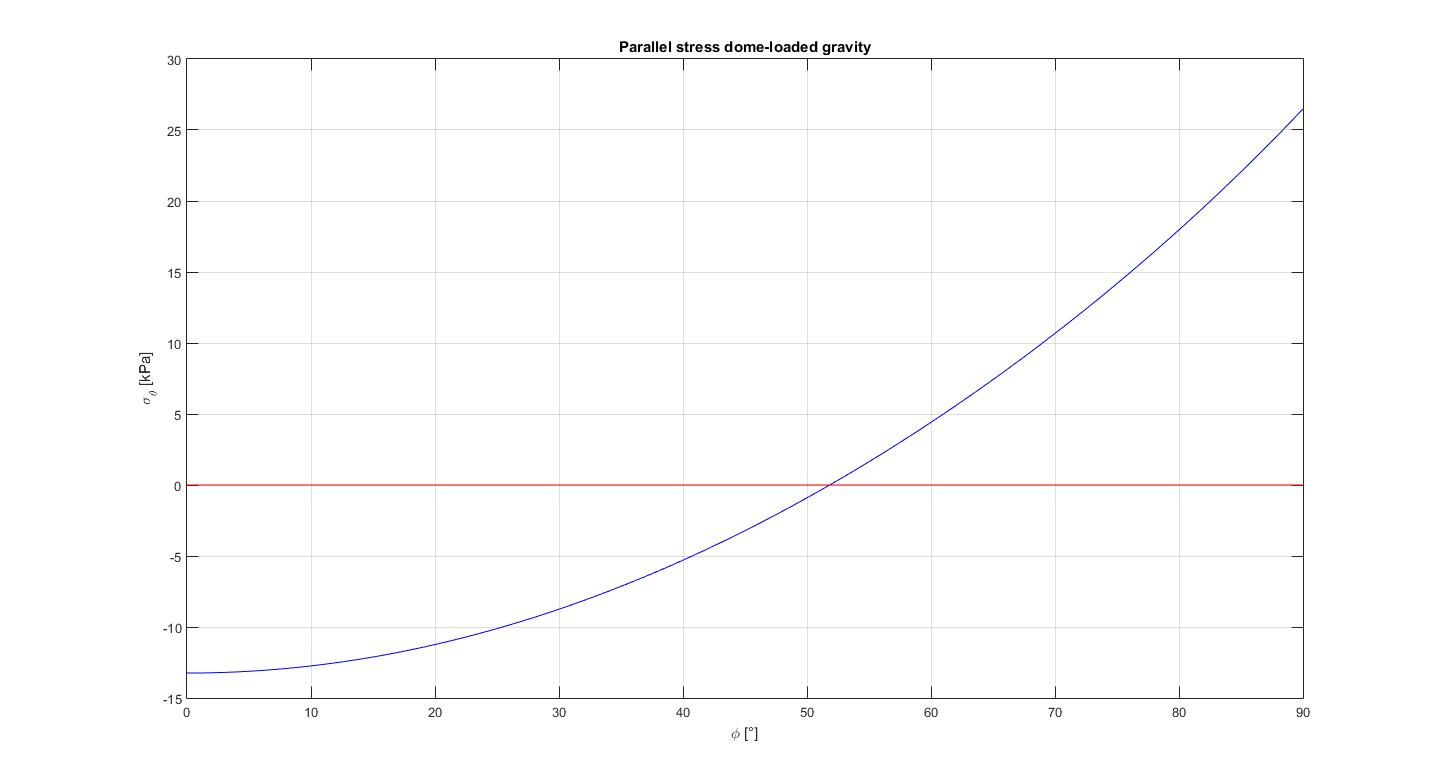
\includegraphics[scale=0.3]{Immagini/gravitateta.jpg}
 	\caption{$\sigma_{\theta}$ al variare di $\phi$}
 \end{figure}
 \begin{figure}[htbp]
 	\centering
 	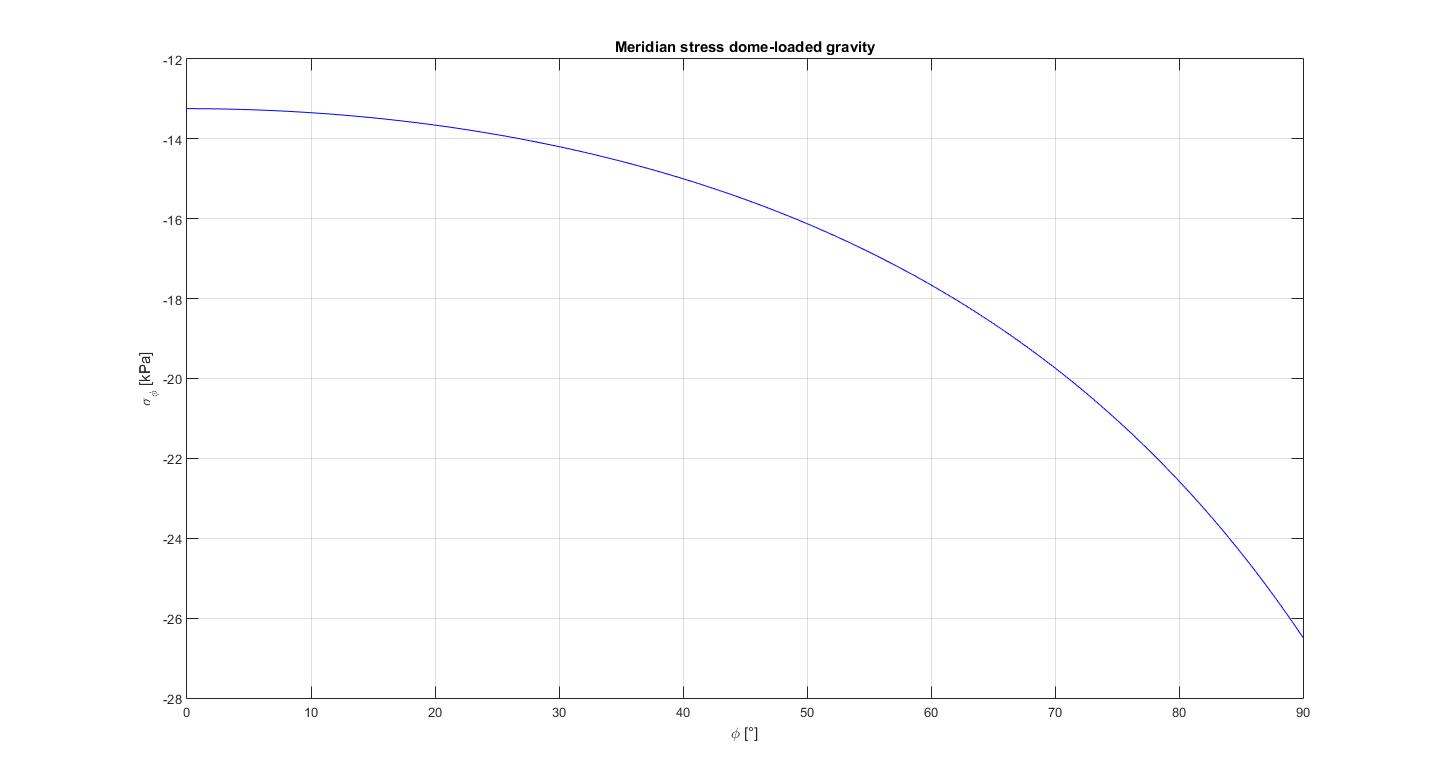
\includegraphics[scale=0.3]{Immagini/gravitafi.jpg}
 	\caption{$\sigma_{\phi}$ al variare di $\phi$}
 \end{figure}
 \newpage
 Si pu\'o notare come la tensione parallela $\sigma_{\theta}$ cambi segno al variare della colatitudine $\phi$ passando da uno stato stress di compressione ad uno di trazione, annullandosi per una $\phi= 51.7�$, infatti per l'elemento 418 ($56� <\phi < 58�$) si ha una $\sigma_{\theta}=1.831168E+03 Pa$ .\\
 Si riportano i risultati sempre in corrispondenza dell'elemento 413, avente come nodi:
 \begin{center}
 	\begin{tabular}{c c}
 		\hline
 		Nodo & Colatitudine $\phi$ \\
 		\hline
 		413 & 46.00� \\ 
 		\hline
 		414 & 44.00� \\ 
 		\hline
 		443 & 46.00� \\ 
 		\hline
 		444 & 44.00�\\  
 		\hline
 	\end{tabular}
 \end{center} 
 	
 	\begin{center}
 		\begin{tabular}{c c}
 			\hline	
 			$\sigma_{\theta_{+}}$ & $ -3.266092E+03 Pa$\\
 			\hline
 			$\sigma_{\theta_{-}}$ & $ -3.144493E+03 Pa$\\
 			\hline
 			$\sigma_{\phi_{+}}$ & $ -1.557026E+04   Pa$\\
 			\hline
 			$\sigma_{\phi_{-}}$ & $ -1.545168E+04   Pa$\\
 			\hline
 		\end{tabular}
 	\end{center} 
 	In perfetto accordo con la teoria analitica; infatti considerando una $\overline{\phi}= 45�$ ovvero la media delle colatitudini dei nodi adiacenti lungo il meridiano, si ottiene $\sigma_{\theta}=-3.213 kPa$ e $\sigma_{\phi}=-15.52 kPa$.
 	Considerando il caso globale, peso pi\'u pressurizzazione si ha:\\
 	\begin{center}
 		\begin{tabular}{c c}
 			\hline
 			Analitico & FEM \\
 			\hline
 			$\sigma_{\theta}=1.8747 MPa$ & $\sigma_{\theta}=1.873688391E+07 Pa$\\
 			\hline
            $\sigma_{\phi}=1.8734 MPa$ & $\sigma_{\phi}=1.872457974E+07 Pa$\\
 			\hline
 		\end{tabular}
 	\end{center}
 
 
Si noti come il carico di gravit\'a influenzi molto poco la soluzione in termini globali.\\
Per completezza si riporta la deformata della struttura.
\begin{figure}[htbp]
	\centering
	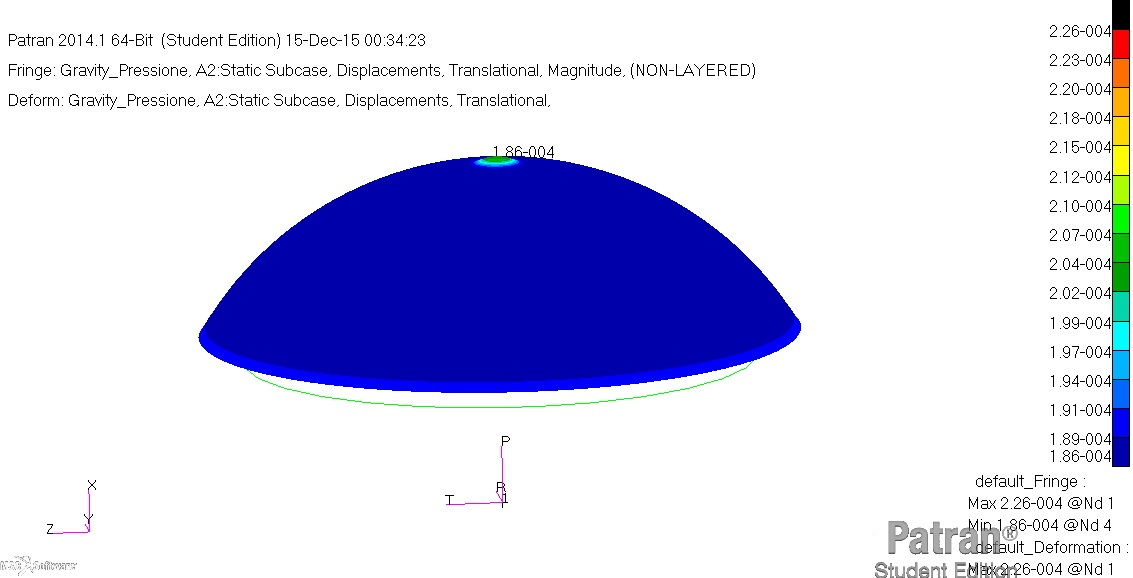
\includegraphics[scale=0.4]{Immagini/Cupolap.jpg}
	\caption{Deformata cupola pressurizzata e sotto azione di gravit\'a}
\end{figure}

 	 
  
 
 
  
 
 
  
 

\subsection{Modi}
Sempre con riferimento alla cupola, si vogliono calcolare i primi 10 modi propri di vibrare; quest'ultimi e le rispettive frequenze sono stati calcolati usando un solutore FEM (SOL 103),  normalizzando tali modi rispetto allo spostamento massimo (MAX) in modo da ottenere uno spostamento massimo pari a 1.\\
Si riportano in tabella i valori delle pulsazioni ottenute tramine Nastran.


\begin{center}
	\begin{tabular}{c c}
		\hline
		Modo & f [Hz] \\
		\hline
       1 & 698.609500 \\ 
       2 & 698.609500 \\ 
       3 & 718.430952 \\ 
       4 & 772.469800 \\ 
       5 & 772.469800 \\ 
       6 & 776.658800 \\ 
       7 & 776.658800 \\ 
       8 & 780.307100 \\ 
       9 & 788.243000 \\ 
       10 & 788.243100 \\ 
		\hline
	\end{tabular}
\end{center}
Vengono riportate le prime 10 deformate.\\
Si noti come le frequenza proprie risultano essere le stesse a coppie, es 1 e 2, e le rispettive deformate modali risultano essere coincidenti ma ruotate spazialmente di un angolo di 90�, questo \'e dovuto alla simmetria della struttura, che in quanto tale non predilige una direzione specifica, questo conduce ad avere delle armoniche trasversali coincidenti.

\begin{figure}[htbp]
	\subfloat[][\emph{Modo 1}.]
	{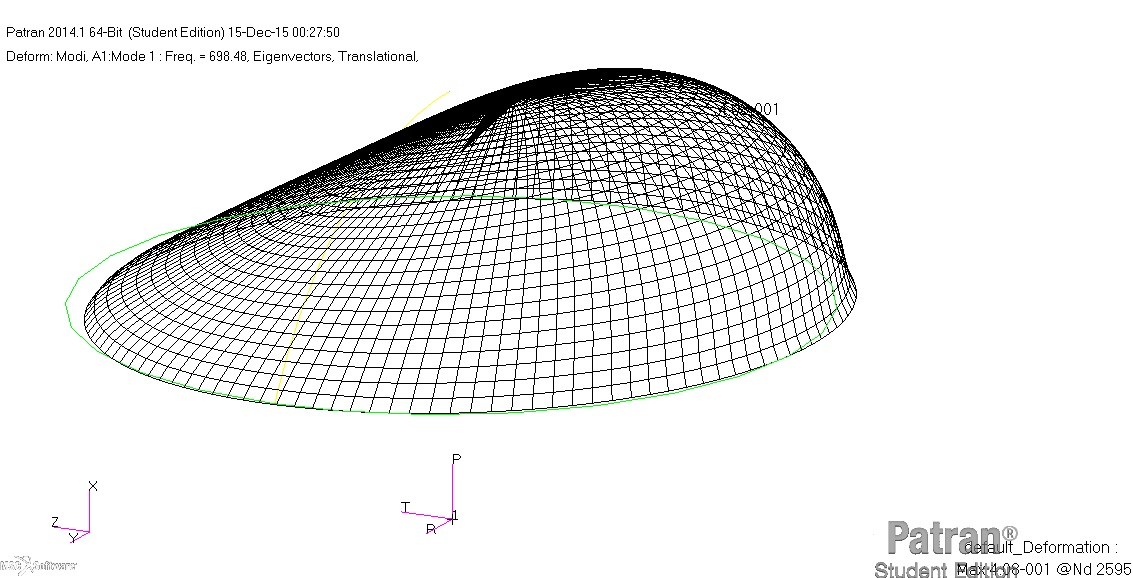
\includegraphics[width=.55\textwidth]{Immagini/modo1c.jpg}} \quad
	\subfloat[][\emph{Modo 2}.]
	{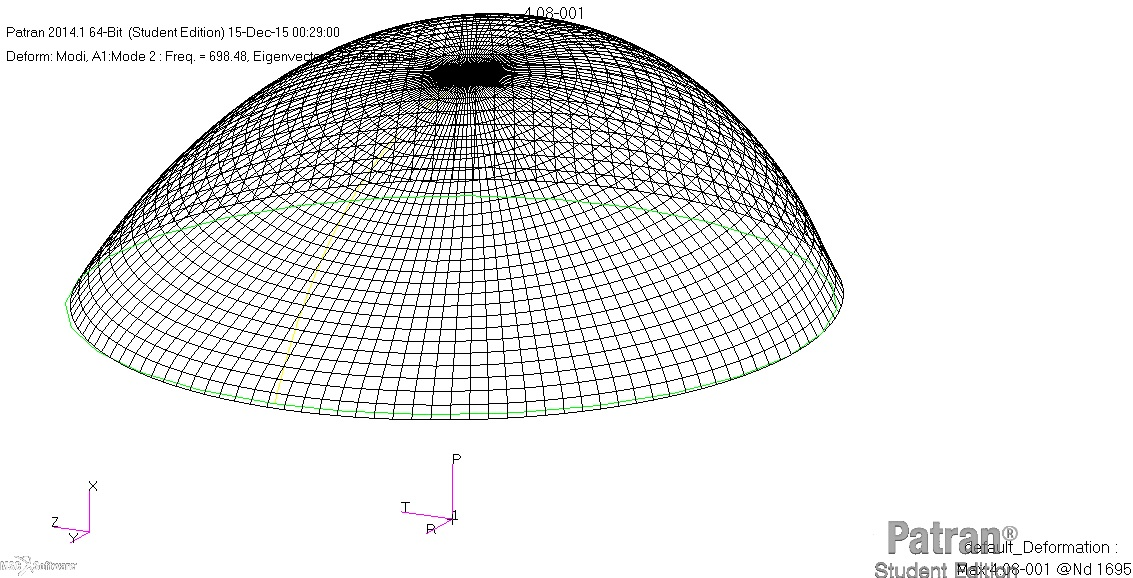
\includegraphics[width=.55\textwidth]{Immagini/modo2c.jpg}} 
	\label{fig:subfig}
\end{figure}
\begin{figure}[htbp]
	\centering
	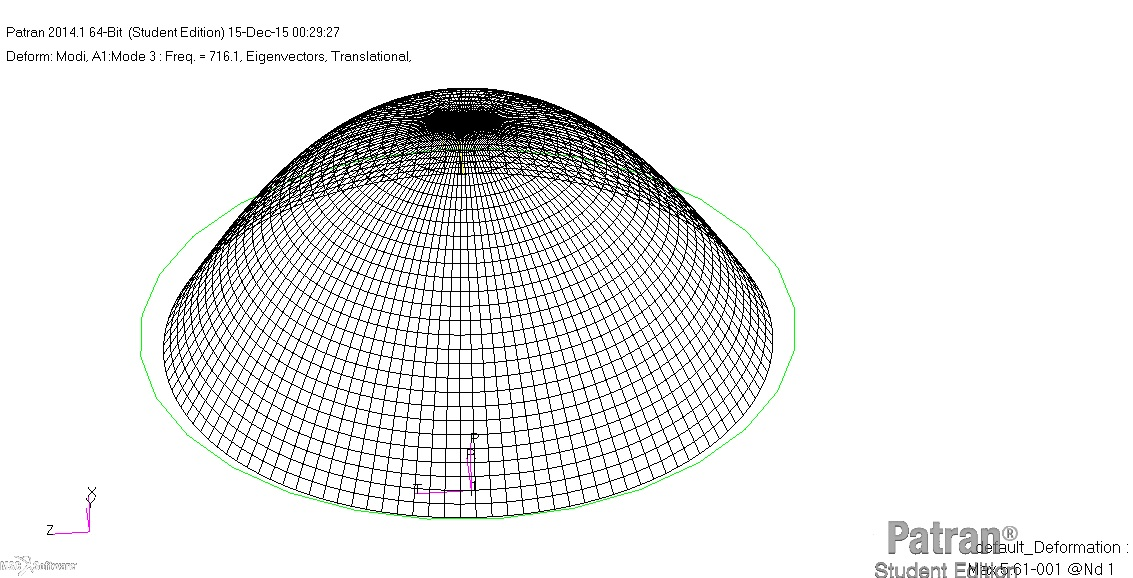
\includegraphics[scale=0.28]{Immagini/modo3c.jpg}
	\caption{Modo 3}
\end{figure}
\begin{figure}[htbp]
	\subfloat[][\emph{Modo 4}.]
	{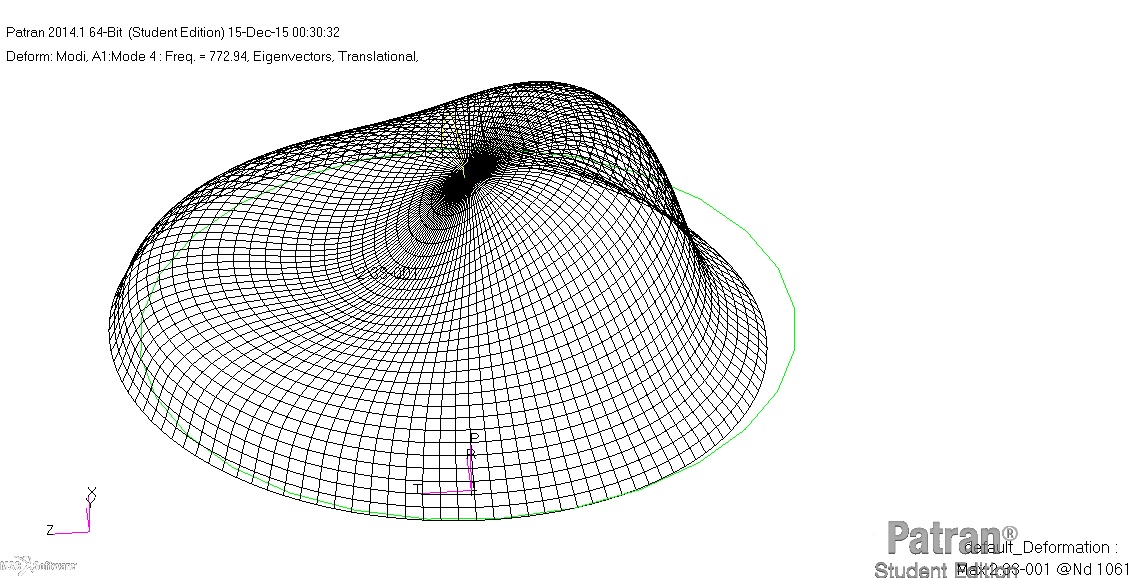
\includegraphics[width=.55\textwidth]{Immagini/modo4c.jpg}} \quad
	\subfloat[][\emph{Modo 5 }.]
	{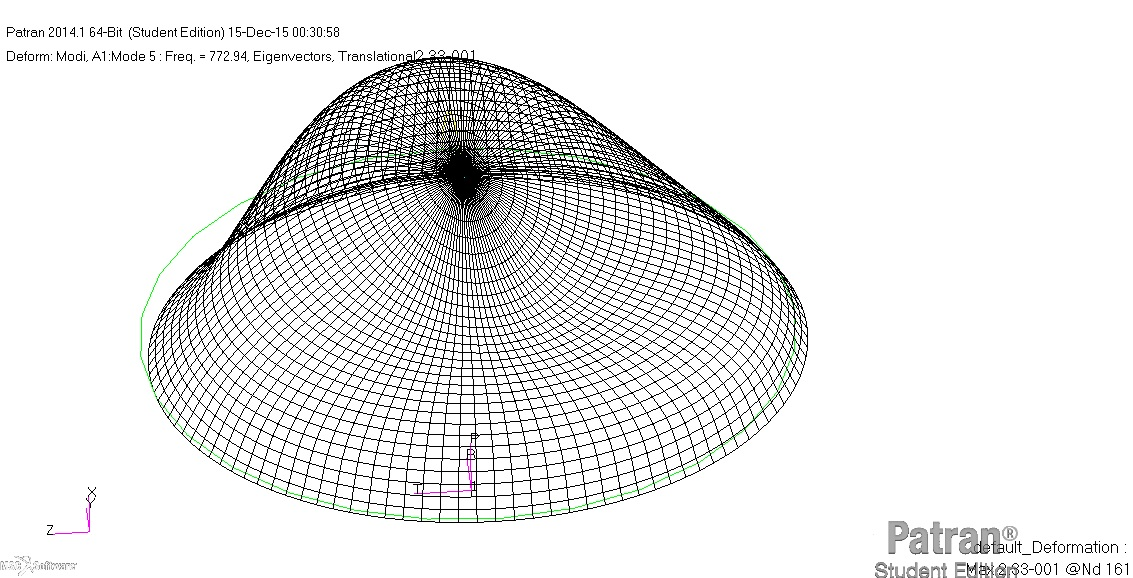
\includegraphics[width=.55\textwidth]{Immagini/modo5c.jpg}} 
	\label{fig:subfig}
\end{figure}
\begin{figure}[htbp]
	\subfloat[][\emph{Modo 6 }.]
	{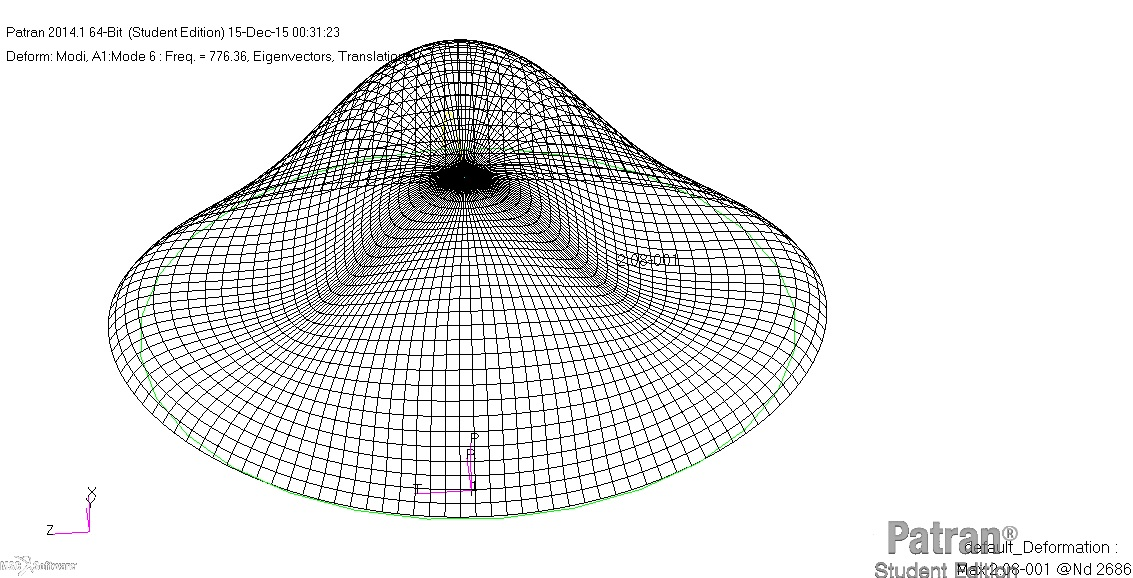
\includegraphics[width=.55\textwidth]{Immagini/modo6c.jpg}} \quad
	\subfloat[][\emph{Modo 7 }.]
	{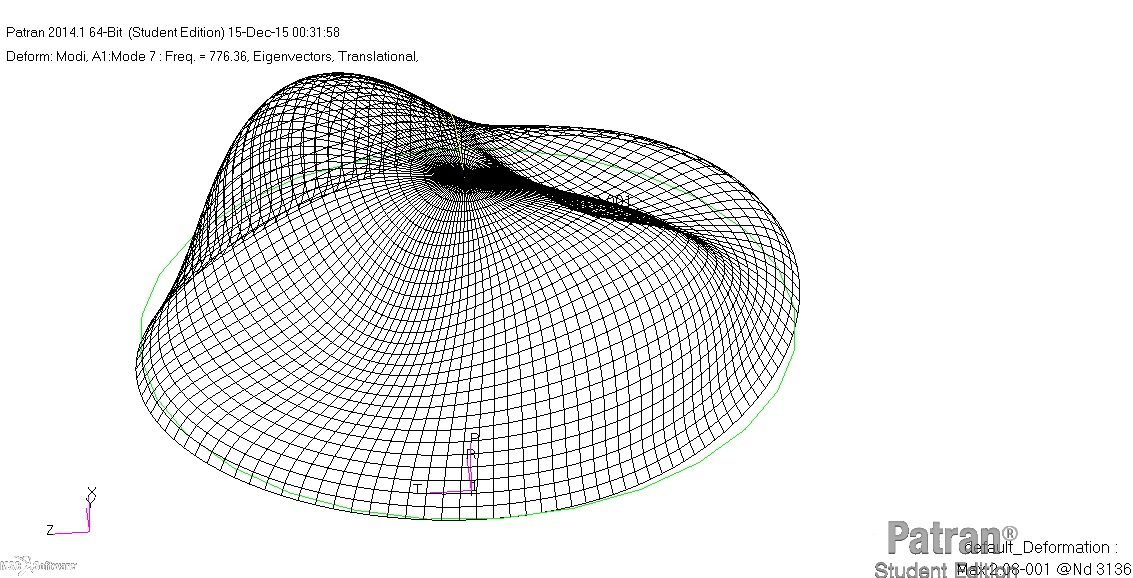
\includegraphics[width=.55\textwidth]{Immagini/modo7c.jpg}} 
	\label{fig:subfig}
\end{figure}
\begin{figure}[htbp]
	\centering
	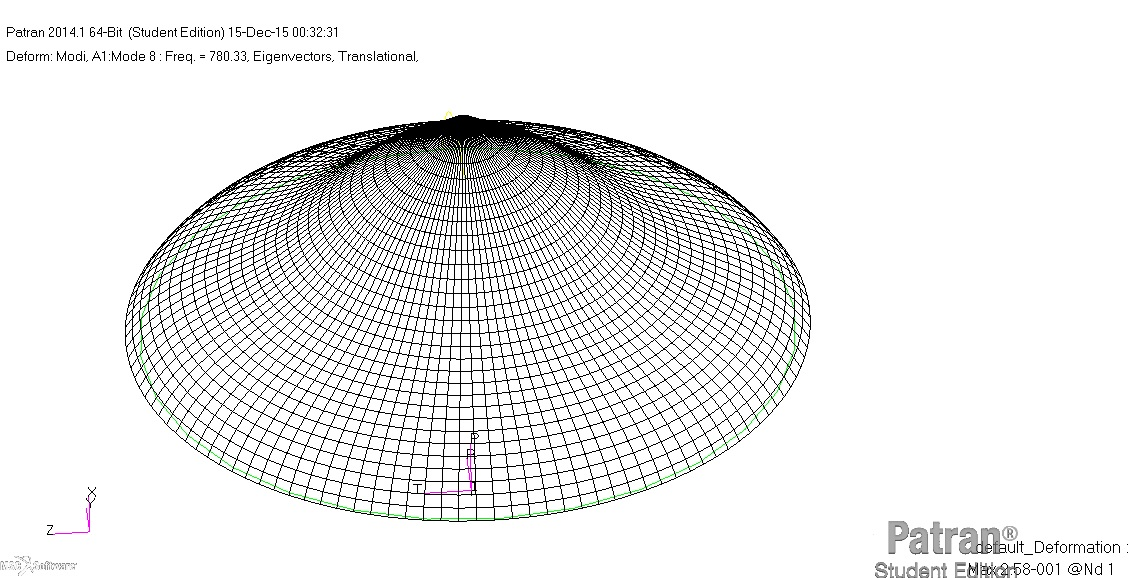
\includegraphics[scale=0.28]{Immagini/modo8c.jpg}
	\caption{Modo 8}
\end{figure}
\begin{figure}[htbp]
	\subfloat[][\emph{Modo 9 }.]
	{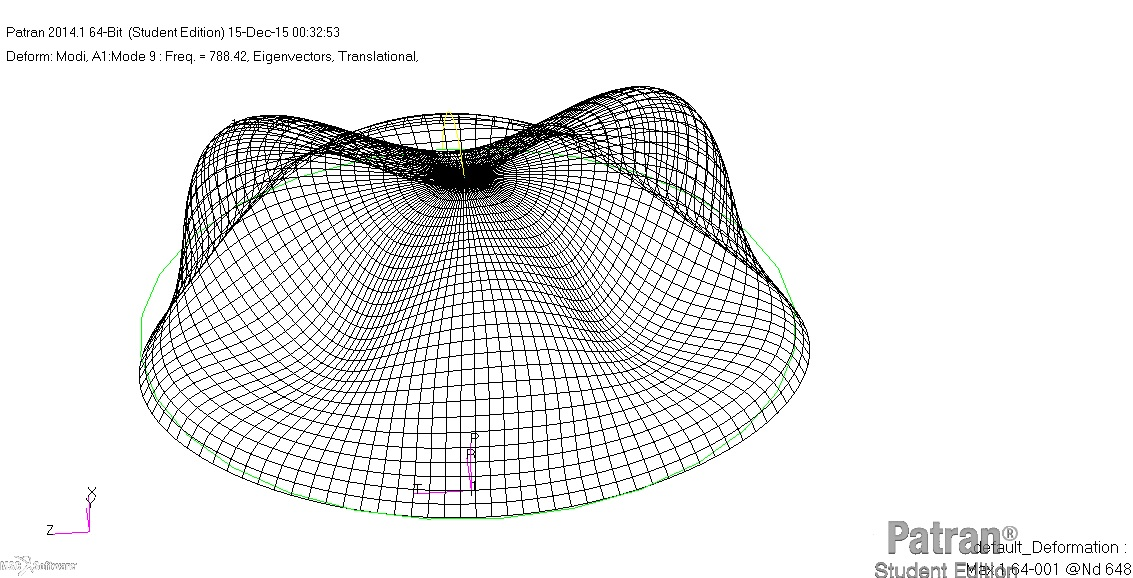
\includegraphics[width=.55\textwidth]{Immagini/modo9c.jpg}} \quad
	\subfloat[][\emph{Modo 10 }.]
	{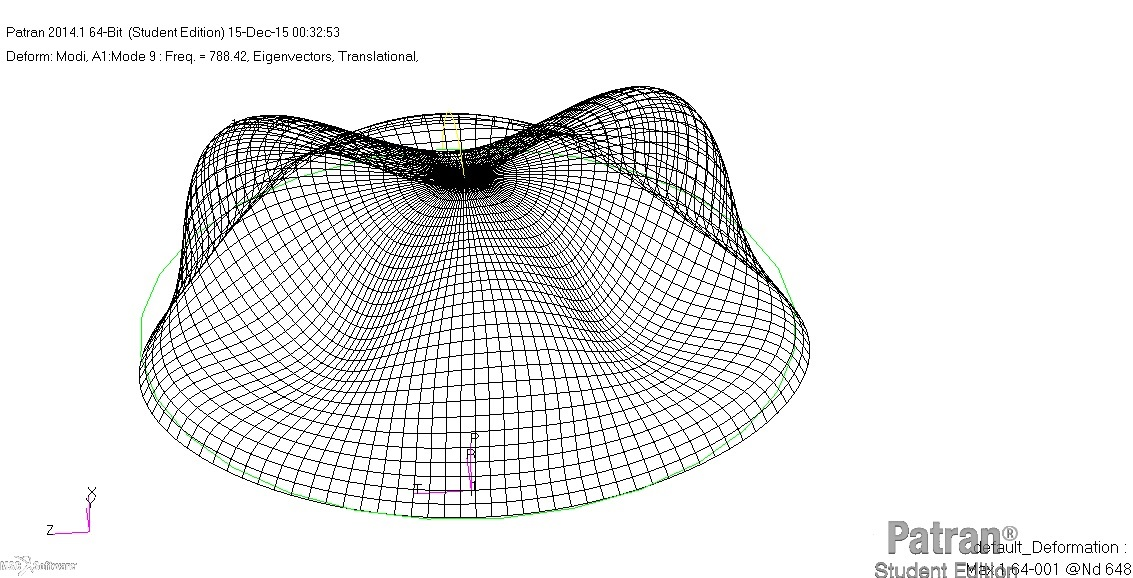
\includegraphics[width=.55\textwidth]{Immagini/modo10c.jpg}} 
	\label{fig:subfig}
\end{figure}
\newpage




\section{Calotta sferica con apertura polare soggetta a carico anulare sulla sommit\'a e peso proprio}
Si vuole determinare la risposta statica della cupola precedentemente trattata, con l'aggiunta di un'apertura polare pari a $\phi_{0}=30�$ (si veda figura), caricata sulla sommit\'a con un carico uniformente distribuito sul bordo di intensit\'a $P=8000 \dfrac{N}{m}$ e soggetta al proprio peso.
\begin{figure}[htbp]
	\centering
	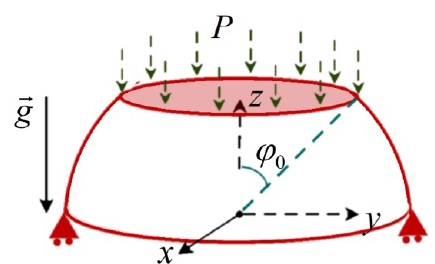
\includegraphics[scale=0.4]{Immagini/Cupolaforata.jpg}
	\caption{Cupola forata}
\end{figure}\\
La soluzione analitica fornisce i seguenti risultati:\\ \\
\textbullet \quad$ \sigma_{\phi}=-\dfrac{\overline{p}\cdot r}{t}\cdot( \dfrac{\cos\phi_{0}-\cos\phi}{\sin^{2}\phi} ) -\dfrac{P\cdot\sin\phi_{0}}{t\cdot\sin^{2}\phi}$ \\ \\
\textbullet \quad $ \sigma_{\theta}=\dfrac{\overline{p}\cdot r}{t}\cdot( \dfrac{\cos\phi_{0}-\cos\phi}{\sin^{2}\phi} -\cos\phi ) -\dfrac{P\cdot\sin\phi_{0}}{t\cdot\sin^{2}\phi}$ \\ \\
La struttura \'e stata discretizzata con 120 elementi lungo ogni parallelo e 30 elementi lungo ogni meridiano (elementi di tipo SHELL). \\Inoltre si \'e sostituita la distribuzione di carico P sul bordo, con un carico equivalente $\overline{F}= P\cdot 2\cdot\pi\cdot r_{0}$, dove $r_{0}=r\cdot\sin(30�)$, ovvero un carico $F=25.133 kN$, applicando quindi un carico concentrato pari a $f=209.44 N$ su ognuno dei 120 nodi distribuiti sul bordo della sommit\'a.\\
Scegliendo come elemento da analizzare il 405 avente nodi: 

\begin{center}
	\begin{tabular}{c c}
		\hline
		Nodo & Colatitudine $\phi$ \\
		\hline
		418 & 44.00� \\ 
		\hline
		419 & 46.00� \\
		\hline 
		449 & 44.00� \\ 
		\hline
		450 & 46.00�\\  
		\hline
	\end{tabular} 
\end{center}  
	si ha che:\\
	
\begin{center}
		\begin{tabular}{c c}
			\hline	
			$\sigma_{\theta}$ & $ -3.797657E+06Pa$\\
			\hline
			$\sigma_{\phi}$ & $ -3.964583E+06 Pa$\\
			\hline
		\end{tabular}
  \end{center} 
  
  Al solito, prendendo una $\overline{\phi}=45.5�$ media tra le due colatitudini dei nodi dell'elemento sul meridiano, la soluzione analitica fornisce $\sigma_{\theta}= -3.9401 MPa$ e $\sigma_{\phi}= -3.9414 MPa$;in buon accordo con la teoria analitica.\\
  Valutando, invece, lo stress su un elemento (elemento 150) in prossimit\'a della sommit\'a, e indicando con + la fibra superiore dello spessore e con - quella inferiore si ha:
  \begin{center}
  	\begin{tabular}{c c}
  		\hline	
  		$\sigma_{\theta_{-}}$ & $ 4.865439E+07 Pa$\\
  		\hline
  		$\sigma_{\theta_{+}}$ & $ -5.732001E+07 Pa$\\
  		\hline
  		$\sigma_{\phi_{-}}$ & $ 1.339110E+08 Pa$\\
  		\hline
  		$\sigma_{\phi_{-}}$ & $ 1.493172E+08 Pa$\\
  		\hline
  	\end{tabular}
  \end{center}   
  Mentre la soluzione analitica fornisce, per $\overline{\phi}=31.5�$ una $\sigma_{\theta}= -7.3272 MPa$ e $\sigma_{\phi}= -7.3472 MPa$, si vede un forte disaccordo con le due soluzioni, si passa da un ordine di grandezza di $10^6$ a uno di $10^8$, questo perch\'e localmente gli effetti flessionali, dovuti alle forte variazioni di curvatura a causa del carico applicato, diventano molto importanti: si noti infatti addirittura il cambio di segno della $\sigma_{\theta}$ nello spessore, si deduce quindi che il range di applicabilit\'a della soluzione analitica ottenuta con la teoria dei gusci sottili sia limitato, per questo tipo di problema. \\
  Si riporta infine la deformata.\\
   \begin{figure}[htbp]
   	\centering
   	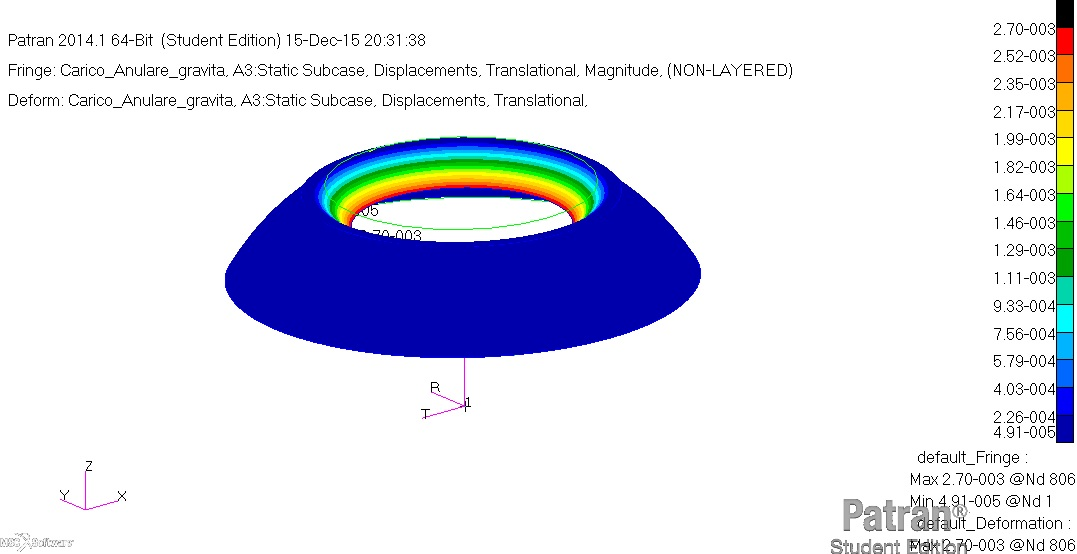
\includegraphics[scale=0.4]{Immagini/Cupolaf.jpg}
   	\caption{Deformata cilindro}
   \end{figure}
\newpage
\subsection{Modi}
L'ultimo caso prevede il calcolo dei modi propri di vibrare; quest'ultimi e le rispettive frequenze sono state calcolate tramite solutore FEM (SOL 103), normalizzando tali modi rispetto allo spostamento massimo (MAX)in modo da ottenere uno spostamento massimo pari a 1.\\
Si riportano in tabella i valori delle frequenze ottenute tramine Nastran.
\begin{center}
	\begin{tabular}{c c}
		\hline
		Modo & f [Hz] \\
      \hline
       1 & 88.813420 \\ 
       2 & 88.813450 \\ 
       3 & 103.431200 \\ 
       4 & 103.431300 \\ 
       5 & 123.111500 \\ 
       6 & 123.111600 \\ 
       7 & 134.664800 \\ 
       8 & 134.665100 \\ 
       9 & 171.755100 \\ 
       10 & 171.755100 \\ 
\hline
\end{tabular}
\end{center}
Vengono riportate le prime 10 deformate.\\
Analogamente a quanto visto precedentemente per i modi e le frequenze proprie della cupola sferica, anche qui si osserva il fatto che le frequenze coincidano a coppie e che le deformate corrispondenti concidano a meno di una rotazione di 90�.\\
\begin{figure}[htbp]
	\subfloat[][\emph{Modo 1}.]
	{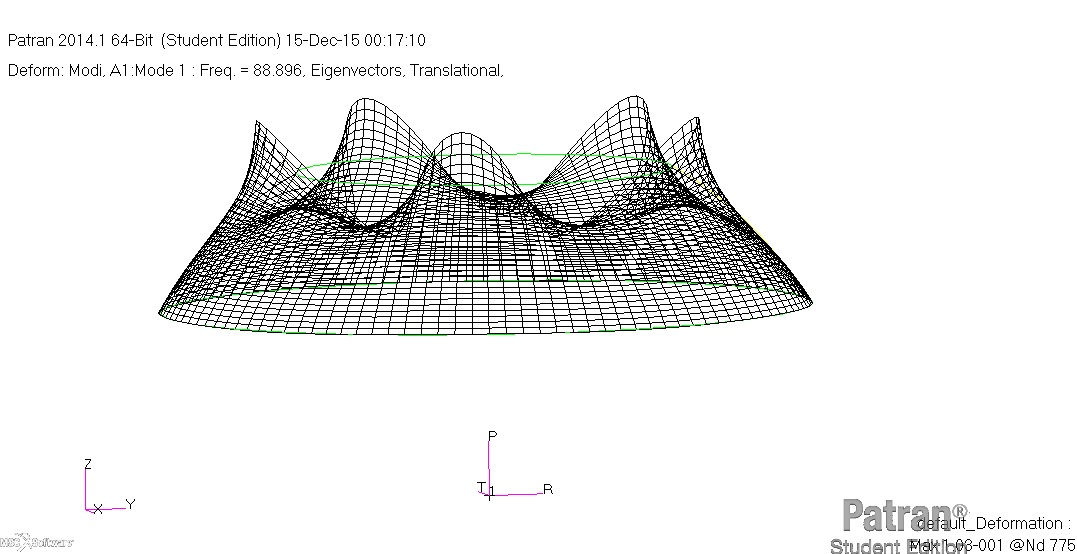
\includegraphics[width=.55\textwidth]{Immagini/modo1.jpg}} \quad
	\subfloat[][\emph{Modo 2}.]
	{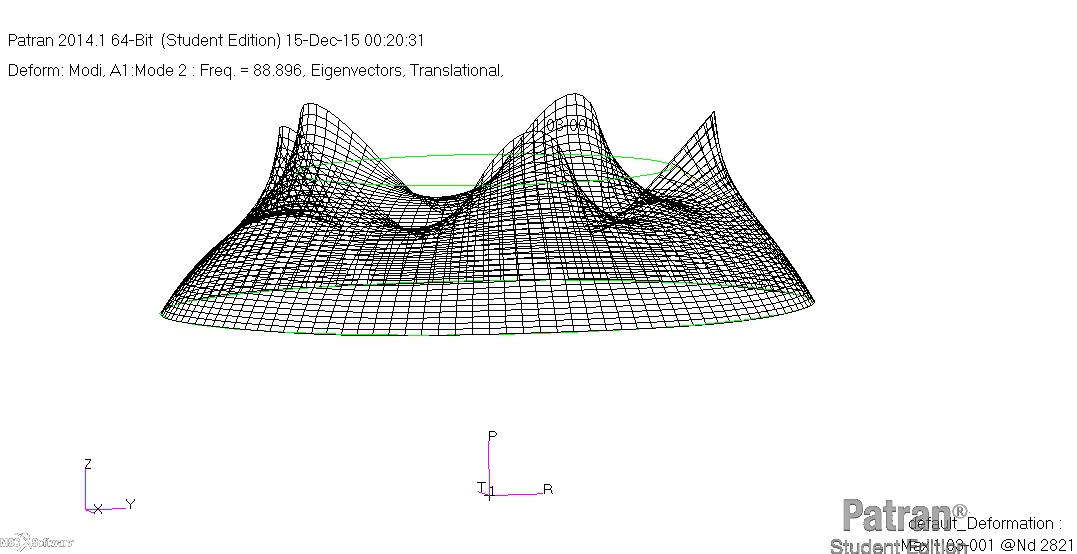
\includegraphics[width=.55\textwidth]{Immagini/modo2.jpg}} 
	\label{fig:subfig}
\end{figure}
\begin{figure}[htbp]
	\subfloat[][\emph{Modo 3}.]
	{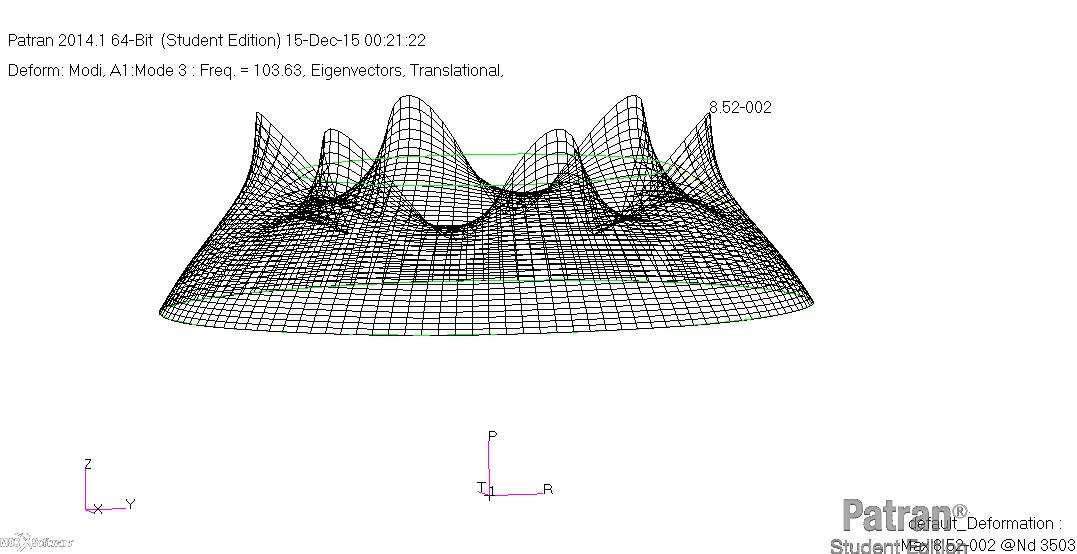
\includegraphics[width=.55\textwidth]{Immagini/modo3.jpg}} \quad
	\subfloat[][\emph{Modo 4 }.]
	{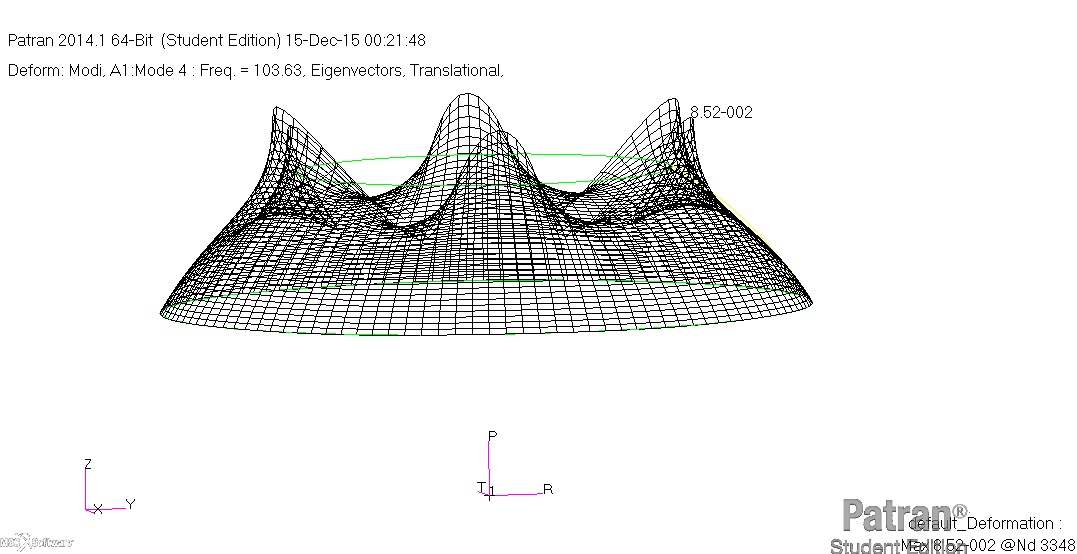
\includegraphics[width=.55\textwidth]{Immagini/modo4.jpg}} 
	\label{fig:subfig}
\end{figure}
\begin{figure}[htbp]
	\subfloat[][\emph{Modo 5 }.]
	{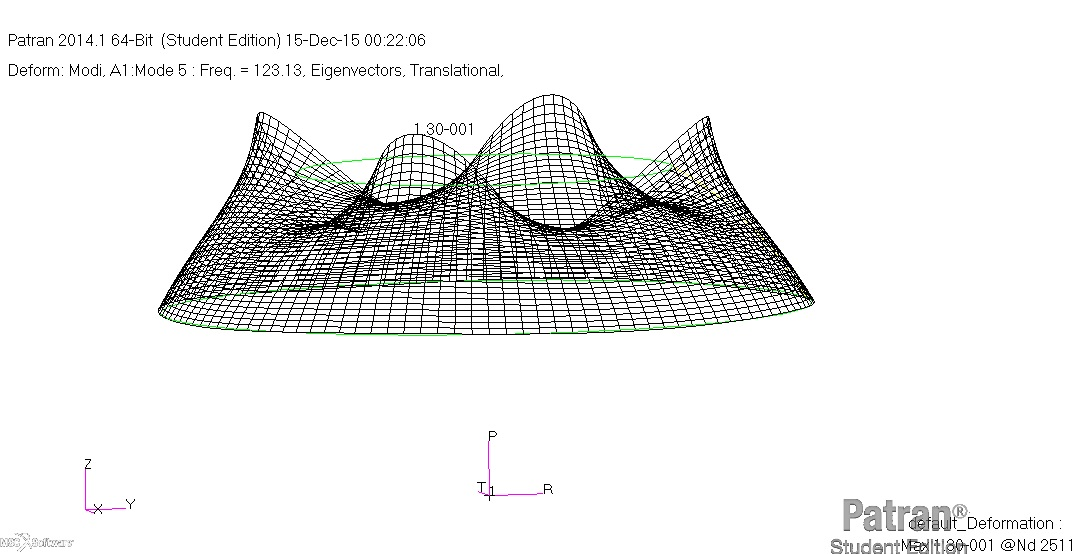
\includegraphics[width=.55\textwidth]{Immagini/modo5.jpg}} \quad
	\subfloat[][\emph{Modo 6 }.]
	{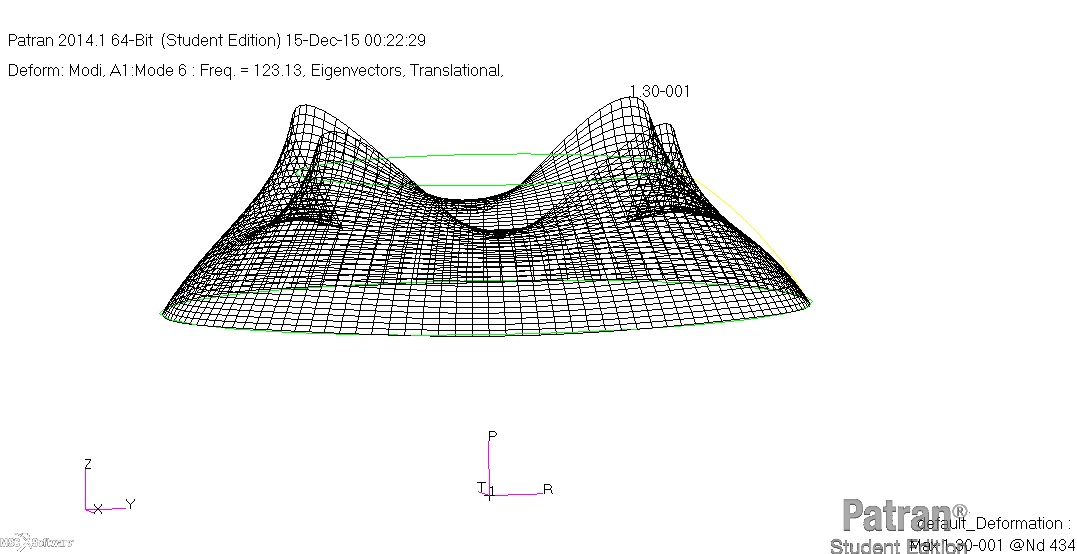
\includegraphics[width=.55\textwidth]{Immagini/modo6.jpg}} 
	\label{fig:subfig}
\end{figure}
\begin{figure}[htbp]
	\subfloat[][\emph{Modo 7 }.]
	{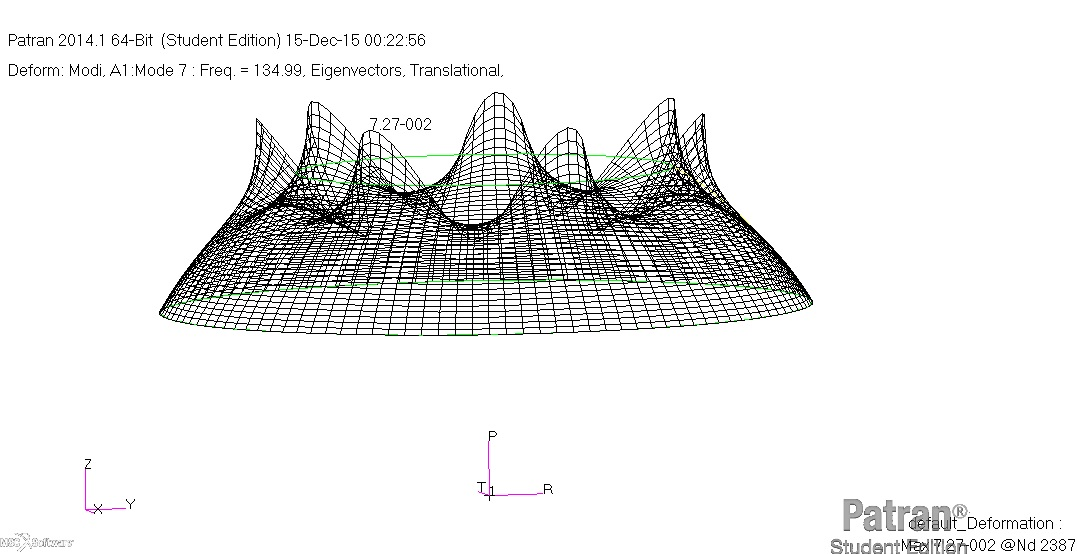
\includegraphics[width=.55\textwidth]{Immagini/modo7.jpg}} \quad
	\subfloat[][\emph{Modo 8 }.]
	{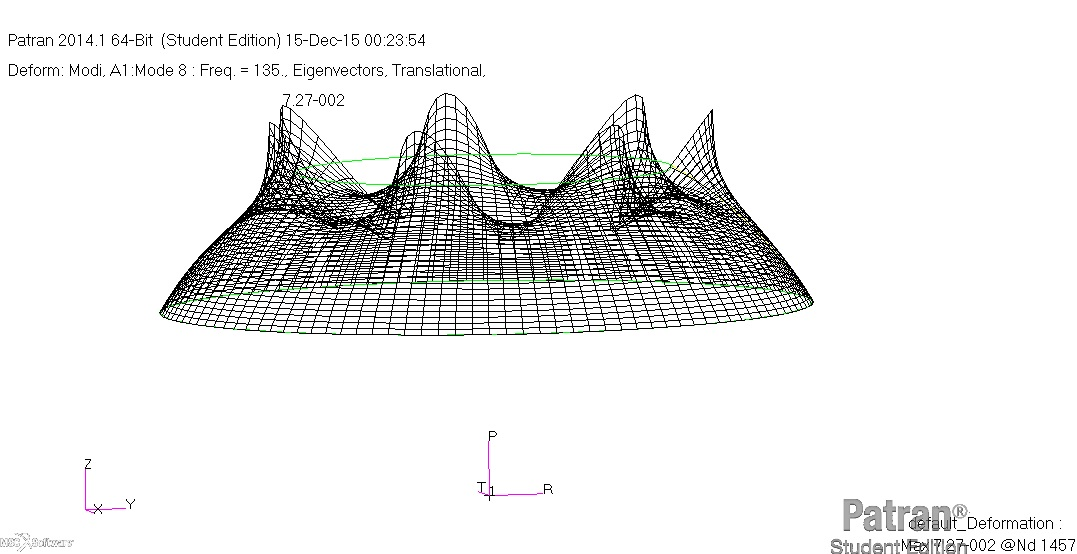
\includegraphics[width=.55\textwidth]{Immagini/modo8.jpg}} 
	\label{fig:subfig}
\end{figure}
\begin{figure}[htbp]
	\subfloat[][\emph{Modo 9 }.]
	{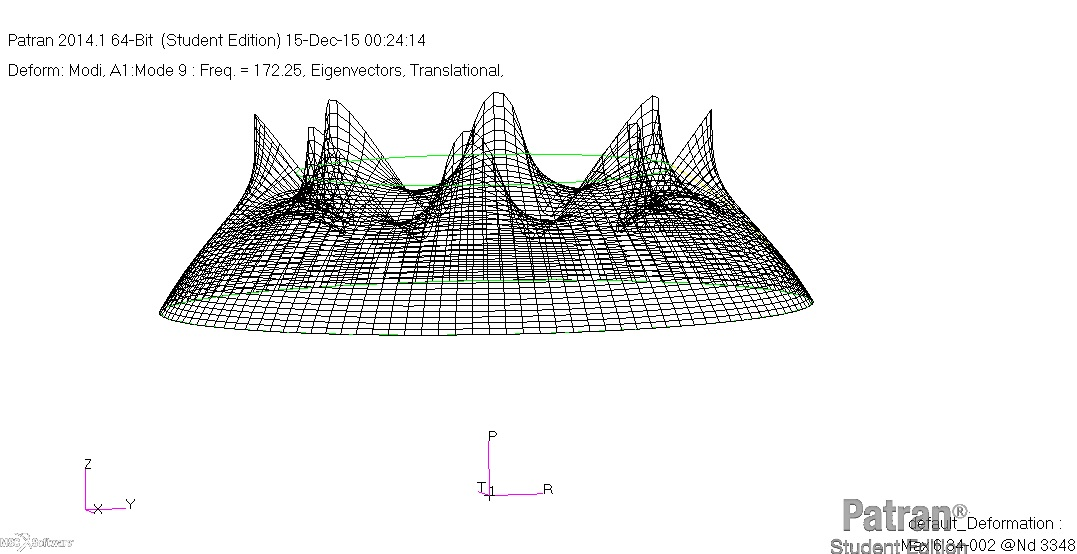
\includegraphics[width=.55\textwidth]{Immagini/modo9.jpg}} \quad
	\subfloat[][\emph{Modo 10 }.]
	{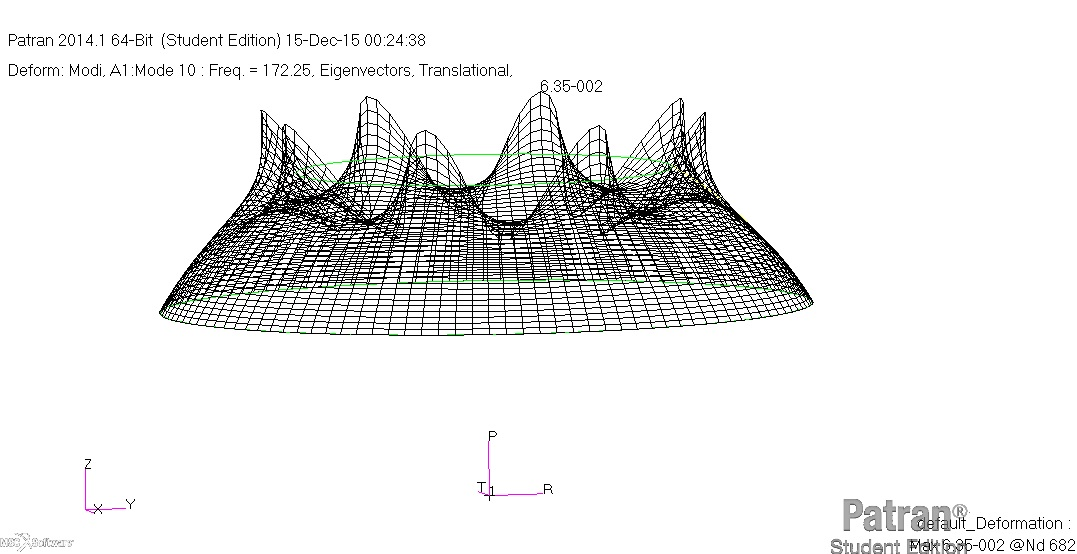
\includegraphics[width=.55\textwidth]{Immagini/modo10.jpg}} 
	\label{fig:subfig}
\end{figure}



\end{document}